\documentclass[10pt]{article}

% Pacotes extras necessários
\usepackage{amsmath}
\usepackage[lmargin=0.5in, rmargin=0.5in, tmargin=0.5in, bmargin=0.5in, includehead, includefoot]{geometry}
\usepackage{amsfonts}
\usepackage[utf8]{inputenc}
\usepackage[portuguese]{babel}
\usepackage{graphicx}
\usepackage{fancyhdr}
\usepackage{setspace}

\graphicspath{ {./images/} }

% Sets para outras partes
\setlength{\parindent}{0pt}
\setstretch{1.5}
\DeclareMathOperator{\sen}{sen}

%% Facilidades
%% -- Laplace
\newcommand{\Lap}[1]{\mathcal{L}\left\{#1\right\}}

%% -- Fourier
\newcommand{\Fou}[1]{\mathcal{F}\left\{#1\right\}}

%% -- Transformada Z
\newcommand{\Z}[1]{\mathcal{Z}\left\{#1\right\}}

%% -- Negrito em matemáticas
\newcommand{\bm}[1]{\boldsymbol{#1}}


% ------- Estilo do trabalho -------- %
\fancypagestyle{capa}{
    \fancyhf{}
    \renewcommand\headrulewidth{0pt}
    \fancyfoot[C]{
        Rio de Janeiro\\
        2022
    }
}

\pagestyle{fancy}
\fancyhead{}
\fancyhead[L]{\thepage}
\fancyfoot{}
% ----------------------------------- %

% Dados do Grupo
\title{Sinais e Sistemas - Trabalho 5 - Avaliação 9}
\author{
    \textbf{Grupo 2}\\
    Leonardo Soares da Costa Tanaka\\
    Matheus Henrique Sant Anna Cardoso\\
    Theo Rudra Macedo e Silva
}
\date{}

\begin{document}
\maketitle
\thispagestyle{capa}
\newpage

%% Questão 1 -----------------
\textbf{1.) Um SLIT relaxado é descrito pela equação a diferenças $y_{k + 2} + \alpha y_k = \beta u_{k + 1} + \gamma u_k$.\\
Os dados $(\alpha, \beta, \gamma)$ são: \textbf{G2: }$(-1/4, 1, 2)$;}

Utilizando as constantes do grupo, a equação torna-se: $y_{k + 2} - \frac{1}{4} y_k = u_{k + 1} + 2 u_k$

(a) Encontrar a função de transferência $G(z)$;

\begin{align*}
    y_{k + 2} - \frac{1}{4} y_k = u_{k + 1} + 2 u_k => z^2 Y(z) - \frac{1}{4}Y(z) = z U(z) + 2 U(z) => Y(z) = \frac{z + 2}{z^2 - \frac{1}{4}}U(z)
\end{align*}

\begin{align*}
    G(z) = \frac{z + 2}{z^2 - \frac{1}{4}}
\end{align*}

(b) encontrar polos e zeros e verificar a estabilidade;

\begin{align*}
    Polos => x^2 - \frac{1}{4} = \left(x + \frac{1}{2}\right)\left(x - \frac{1}{2}\right) => p_1 = \frac{1}{2} ; p_2 = -\frac{1}{2}
\end{align*}

\begin{align*}
    Zeros => x + 2 => z_1 = -2
\end{align*}

O SLIT é estável nesse caso, porque seus pólos $p_1$ e $p_2$ estão no círculo unitário.

\vspace{\baselineskip}

(c) encontrar as equações dinâmicas;

\begin{align*}
    x_1[k] = y[k]&& => && x_1[k+1] = y[k+1] = x_2[k] - p_1 u[k] \\
    x_2[k] = y[k+1] + p_1 u[k] && => && x_2[k+1] = y[k+2] + p_1 u[k] = \frac{1}{4} x_1[k] + (p_1 + 1) u[k+1] + u[k]
\end{align*}

\begin{align*}
    p_1 = - 1
\end{align*}

\begin{align*}
    x_1[k] = y[k]&& => && x_1[k+1] = x_2[k] + u[k] \\
    x_2[k] = y[k+1] - u[k] && => && x_2[k+1] = \frac{1}{4} x_1[k] + u[k]
\end{align*}

\begin{align*}
    x[k+1]
    =
    \begin{bmatrix}
        0 && 1 \\
        1/4 && 0
    \end{bmatrix}
    x[k]
    +
    \begin{bmatrix}
        1\\
        1
    \end{bmatrix}
    u[k];
    \quad
    y[k] =
    \begin{bmatrix}
        1 && 0
    \end{bmatrix}
    x[k]
\end{align*}

(d) calcular, iterativamente, os 10 primeiros valores $y_k$ para entrada em degrau unitário;

(e) usando transformada em $Z$, encontrar uma expressão analítica para a $y_k$;

(f) comparar os resultados iterativo e analítico.


\vspace{\baselineskip}


%% Questão 2 ------------------
\textbf{G2: 2.) Eis um ``Problema de Algibeira": um vendedor de queijos efetua apenas transações do tipo \emph{vende metade de seu estoque mais meia peça}. Pede-se o número inicial de peças, $x_0$ se após a 6ª venda seus queijos acabam. Interpretar a filosofia de vendas por meio de uma equação a diferenças e calcular $x_k$, o saldo de estoque após a $k$-ésima venda. Dar a resposta ao problema de algibeira.}

Antes de mais nada, podemos pensar um pouco antes de tomarmos quaisquer decisões. É claro ser impossível realizar a venda de meia peça, portanto, é provável que seja uma correção, justamente para que não se venda meia peça. Veja o processo:

\textbf{Processo: (Venda)}

Após a venda $k$: $c$ peças.

Logo antes: $c + 1/2$ peças.

Antes da venda $k$: $2 \cdot (c + 1/2) = \boxed{2c + 1}$ peças. Ou, após a venda $k - 1$.

Disso, podemos ir dando passos para trás até chegarmos ao momento anterior à primeira venda. Considerando, cada processo, uma venda e que antes de cada venda, teremos $2c + 1$ peças, sendo $c$ o número de peças após essa venda:

Após a venda 6: 0\\
Após a venda 5: $2 \cdot 0 + 1 = 1$\\
Após a venda 4: $2 \cdot 1 + 1 = 3$\\
Após a venda 3: $2 \cdot 3 + 1 = 7$\\
Após a venda 2: $2 \cdot 7 + 1 = 15$\\
Após a venda 1: $2 \cdot 15 + 1 = 31$\\
Finalmente, antes da primeira venda, teremos: $2 \cdot 31 + 1 = 63$

Portanto, com passos simples, podemos resolver este problema.

Ainda assim, é possível resolvê-lo por métodos analíticos, com uma equação a diferenças, modelando da seguinte maneira: a quantidade de peças após a venda $k$ $(x_k)$ é a metade da anterior subtraída de 1/2, da forma abaixo:
\[x_k = \frac{1}{2}x_{k - 1} - \frac{1}{2}\]

Podemos realizar a transformada Z desta equação, obtendo:
\begin{align*}
    \Z{x_k} &= \frac{1}{2} \Z{x_{k - 1}} - \frac{1}{2} \Z{1[k]}\\
    X(z) &= \frac{1}{2} \left(z^{-1} X(z) + x[-1]\right) - \frac{z}{2z - 2}\\
    X(z) \left[\frac{2z - 1}{2z}\right] &= \frac{x[-1]}{2} - \frac{z}{2z - 2}\\
    X(z) \left[\frac{2z - 1}{2z}\right] &= \frac{x[-1](z - 1)}{2z - 2} - \frac{z}{2z - 2}\\
    X(z) \left[\frac{2z - 1}{2z}\right] &= \frac{x[-1]z - x[-1] - z}{2z - 2}\\
    \frac{X(z)}{z} &= \frac{x[-1]z - x[-1] - z}{(z - 1)(2z - 1)}\\
    \frac{X(z)}{z} &= \frac{x[-1] + 1}{2z - 1} - \frac{1}{z - 1}\\
    X(z) &= \frac{x[-1] + 1}{2} \left(\frac{z}{z - 1/2}\right) - \frac{1}{z - 1}
\end{align*}

A partir daqui, podemos fazer a transformada inversa:
\begin{align*}
    x[k] = \frac{x[-1] + 1}{2} \left(\frac{1}{2}\right)^{k} - 1[k]
\end{align*}

Podemos descobrir $x[-1]$ dado que sabemos $x[6]$:
\begin{align*}
    x[6] &= 0 = \frac{x[-1] + 1}{2} \left(\frac{1}{2}\right)^{6} - 1[6]\\
    0 &= \frac{x[-1] + 1}{128} - 1\\
    128 &= x[-1] + 1
\end{align*}
\[\boxed{x[-1] = 127}\]

Temos tudo o que precisamos:
\begin{align*}
    x[k] = \frac{x[-1] + 1}{2} \left(\frac{1}{2}\right)^{k} - 1[k]\\
    x[k] = 64 \left(\frac{1}{2}\right)^k - 1[k]
\end{align*}

Aplicando para $k = 0$, teremos:
\[x[0] = 64 \cdot 1 - 1\]
\[\boxed{x[0] = 63}\]

Que foi o resultado obtido da primeira forma.

\vspace{\baselineskip}

%% Questão 3 --------------------
\textbf{3.) Para a EDLIT $\tau \dot{y}(t) + y(t) = \beta u(t)$ com $y(0^-) = y_0$:\\
\textbf{G2: } $\tau = 2, \beta = 2 \text{ e } y_0 = 1$.}

Utilizando as constantes do grupo, a equação torna-se: $2 \dot{y}(t) + y(t) = 2 u(t)$ com $y(0^-) = 1$

(a) Calcular a resposta à rampa unitária por Laplace, e traçar com precisão o seu gráfico para $t \in [0,\,5\tau]$;

\begin{align*}
    \dot{y}(t) + \frac{1}{2} y(t) = u(t); \quad y(0^-) = 1; \quad u(t) = t1(t) \\
    sY(s) - y(0^-) + \frac{1}{2} Y(s) = \frac{1}{s^2} \\
    (s + 1/2)Y(s) = \frac{s^2 + 1}{s^2} \\
    Y(s) = \frac{s^2 + 1}{s^2(s + 1/2)} = \frac{r_1}{s^2} + \frac{r_2}{s} + \frac{r_3}{s + 1/2} \\
    r_1 = 2; \quad r_2 = -4; \quad r_3 = 5 \\
    Y(s) = \frac{2}{s^2} - \frac{4}{s} + \frac{5}{s + 1/2} \\
    y(t) = 2t \ 1(t) - 4 \ 1(t) + 5e^{-\frac{1}{2} t} 1(t)
\end{align*}

\begin{verbatim}
    %Questão 3.a)

    % Intervalo
    dt=0.001;

    % Dados basicos
    t=0:dt:10-dt; x=2*t-4+5*exp(-1/2*t);
    plot (t, x, "r", "linewidth", 3);
    title("y(t) por t - 3.a)", "fontsize", 20);
    xlabel("t", "fontsize", 18);
    ylabel("y(t)", "fontsize", 18);
\end{verbatim}

\begin{figure}[h]
    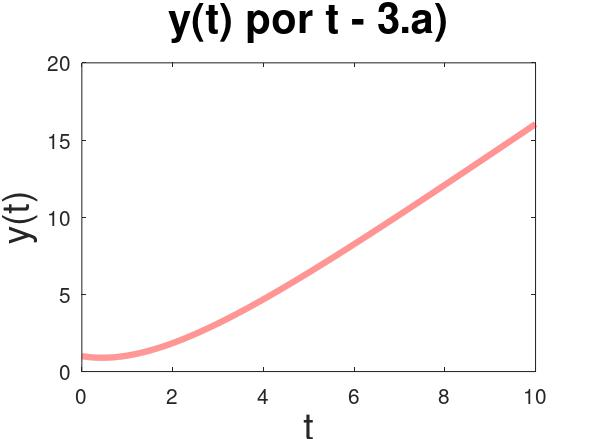
\includegraphics[scale=0.3]{questao3a.jpg}
    \centering
\end{figure}

(b) por Euler I, encontrar a equação que relaciona $y_k \leftrightarrow y(kT)$ e $u_k \leftrightarrow u(kT)$;

(c) resolvê-la por transformada $Z$ para entrada em rampa;

(d) listar as sequências obtidas para $T = \tau, T = \tau / 2, T = \tau / 4 \text{ e } T = \tau / 8$;

(e) plotar os valores de $y(kT)$ no mesmo gráfico do ítem (a) e comparar as aproximações numéricas;

(f) repetir (b), (c), (d) e (e) para Newton.

\vspace{\baselineskip}


%% Questão 4 ----------------------------
\textbf{4.) Para a EDLIT $\ddot{y}(t) + 2\zeta \omega_n \dot{y}(t) = \alpha \dot{u}(t) + \beta u(t)$ com CIs nulas:\\
Os dados $(\zeta,\, \omega_n,\, \beta,\, \alpha)$ são \textbf{G2: }$(1/3,\, 2,\, 3,\, -1)$.}

Utilizando os dados do grupo, temos: $\ddot{y}(t) + \frac{4}{3} \dot{y}(t) = -\dot{u}(t) + 3u(t)$

(a) para $u(t) = 1$, encontre, por Laplace, a solução e plote-a com precisão para $t \in [0,\, 8/(\zeta \omega_n)]$;

(b) por meio de variáveis $x_1$ e $x_2$ apropriadas, expressá-la como $\dot{\bm{x}}(t) = A\bm{x}(t) + B\bm{u}(t)$ e $\bm{y}(t) = C\bm{x}(t) + D\bm{u}(t)$;

(c) por Euler I, relacione $\bm{x}_k \leftrightarrow \bm{x}(kT), \, y_k \leftrightarrow y(kT)$ e $u_k \leftrightarrow u(kT)$ (o procedimento para vetores é o mesmo e leva a $\bm{x}_k = A_d \bm{x}_{k - 1} + B_d \bm{u}_k$ e $\dot{\bm{y}}_k = C_d \bm{x}_k + D_d \bm{u}_k$) e obtenha $y_k$;

(d) plota as sequências obtidas para $T = T_0 = 1 / (\zeta \omega_n), \, T = T_0/2, \, T = T_0/4$ e $T = T_0/8$ no gráfico de (a) e compare as aproximações numéricas.


\vspace{\baselineskip}

%% Questão 5 ------------------------------
\textbf{5.) Seja EDVT $\dot{y}(t) + \alpha(t)y(t) = u(t)$ com $u(t) = 1(t)$. Quando um sinal contínuo $p$ tende a uma constante para valores altos de $t$ ($\lim p(t) = p_r = $ cte. para $t \to \infty$) esta é chamada de valor de regime do sinal.}

(a) sem resolver a equação calcular o valor de regime $y_r$, supondo que $y(t)$ tende a ele;

(b) por Euler I, relacione as sequências $u_k \leftrightarrow u(kT)$ e $y_k \leftrightarrow y(kT)$;

(c) resolva, manualmente ou por meio de um script em alguma linguagem, para $T = 1, T = 1/2, T = 1/4$ e $T = 1/10$; a solução $y(t)$ deve ser aproximada para $t \in [0, \, 10]$;

(d) repetir (b) e (c) para Euler II.

Os dados $a(t)$a e $y(0^-)$ são: \textbf{G2: }$(t^2 - 1)/(t^2 + 1)$ e $-1$.

\end{document}
